
\chapter{La détection mobile}

\label{chapitre2}
		
		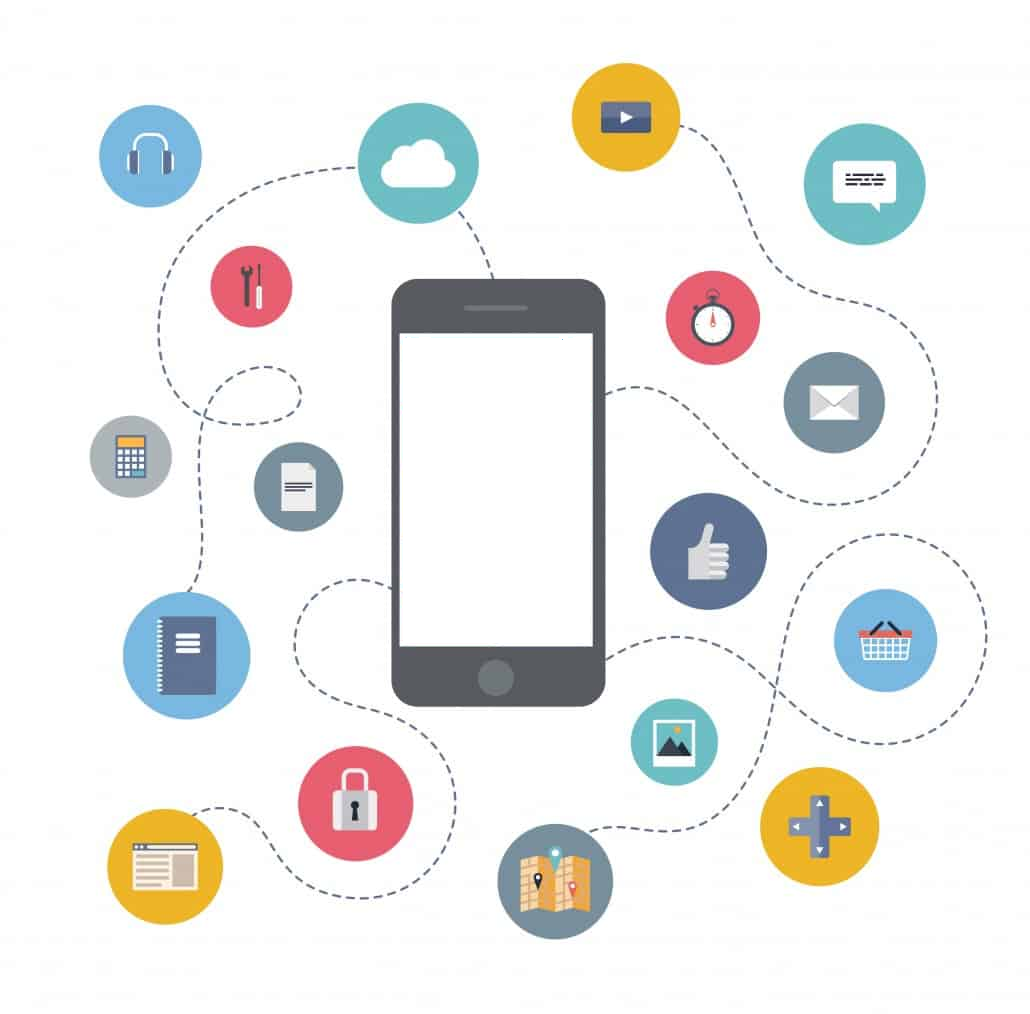
\includegraphics [width=1 \linewidth, height=0.8\textheight, keepaspectratio] {Images/chapterFigures/chTwo.png}
		
	
		
		\newpage

Récemment, des petits capteurs de haute performance se sont répandus et sont intégrés dans divers types d'objets dans notre environnement.

La détection mobile "Mobile sensing" utilise des capteurs intégrés dans des objets en mouvement tels que des voitures, des vélos et des smartphones, puis les considère comme des capteurs de détection \cite{nomuraMethodEstimatingRoad2015}.

De plus, le taux de propagation des smartphones de haute qualité augmente et continuera de le faire. Ces derniers incluent de différents types de capteurs tels que des capteurs d'accélération et des capteurs gyroscopiques.

%---- talking about sensors---%


\section{Différents Capteurs}

Le capteur est un appareil qui détecte les changements dans l'environnement proche et envoie ces données au système d'exploitation ou au processeur. Ils détectent et collectent les données pour lesquelles ils sont faits.

Il existe trois catégories principales de capteurs que possède un smartphone \cite{tilluMobileSensorsComponents2019}:

{\bf Les capteurs de mouvements:}
ils mesurent les forces d'accélération et les rotations autour des trois axes.  Ces capteurs sont capables de déterminer dans quelle direction est orienté l’appareil. A titre d’exemple, On trouve l'accéléromètre et le gyroscope.

    {\bf Les capteurs de position et d’attitude:}
Ce genre de capteurs détermine la position et l’orientation de l'appareil. On trouve donc les capteurs d’orientation, le gyroscope et le magnétomètre ainsi que le GPS.

    {\bf Les capteurs environnementaux:}
c’est des capteurs qui mesurent la pression atmosphérique, l'illumination et la température ambiante (Baromètre, photomètre et thermomètre).

\section{Capteurs d'un smartphone}

\subsection{Accéléromètre}
L'accéléromètre détecte les changements d'orientation des smartphones par rapport aux 3 axes orthogonaux (X, Y et Z). Cette accélération est utilisée pour déterminer la vitesse de l’appareil.

\begin{figure}[h!]
    \center
    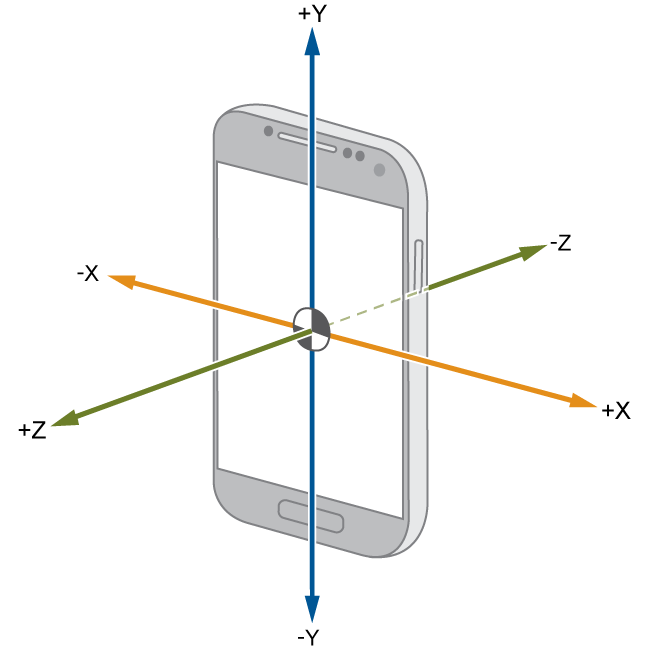
\includegraphics[width=0.60\textwidth]{Images/chapter1/axes.png}
    \caption{Axes orthogonaux utilisés}
    \label{fig:axis}
\end{figure}

\subsection{Gyroscope}
Le gyroscope ou capteur gyroscopique est une version avancée de l'accéléromètre. Alors que l'accéléromètre détecte la détection de mouvement basée sur l'axe, le gyroscope fonctionne avec l'accéléromètre et détecte chaque degré de changement d'orientation. Il fournit une détection de mouvement très précise.

\subsection{GPS}
Le GPS ou le système de positionnement global est également très courant dans la plupart des téléphones modernes. Il aide à localiser l'emplacement sur Terre et aide à la navigation.

\section{Applications utilisant la détection mobile.}
Avec l'évolution des smartphones, le monde a commencé à tirer de plus en plus d'avantages de leurs capacités pour développer de nombreuses applications mobiles. Dont certaines faisant usage des capteurs du smartphone pour réaliser et automatiser des tâches qui étaient avant impossibles sans des appareils sophistiqués.
\subsection{Galaxy Watch}
Galaxy Watch est une montre intelligente développée par Samsung Electronics. Elle embarque une multitude de capteurs : Accéléromètre, baromètre, capteur gyroscopique, capteur cardiaque électrique (ECG), capteur de fréquence cardiaque optique et un capteur de lumière.

Le capteur de fréquence cardiaque mesure votre fréquence cardiaque en battements par minute à l'aide d'une source de lumière LED optique et d'un capteur de lumière LED. La lumière brille à travers votre peau et le capteur mesure la quantité de lumière réfléchie. Les reflets de la lumière varient au fur et à mesure que le sang pulsera sous votre peau au-delà de la lumière.
\begin{figure}[h!]
    \center
    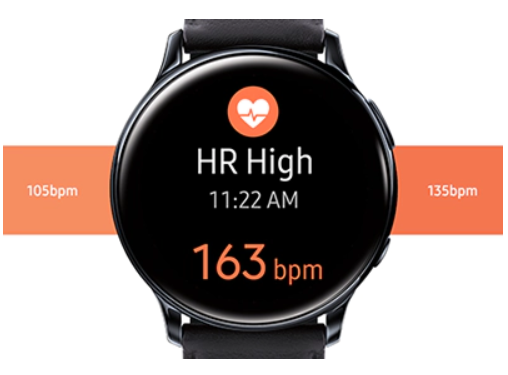
\includegraphics[width=0.5\textwidth]{Images/chapter1/galaxyWatch.PNG}
    \caption{Galaxy Watch}
    \label{fig:Application}
\end{figure}
\subsection{Uber}
Uber est un service de voiture à la demande qui vous permet de demander les services d'un chauffeur privé grâce à une application fonctionnant sur iPhone et Android. Ce service utilise un logiciel qui permet d'envoyer au chauffeur le plus proche votre localisation.

La cartographie est un élément clé du service de VTC (Voiture de transport avec chauffeur). Les opérateurs locaux d'Uber doivent en effet pouvoir visualiser en temps réel les chauffeurs qui circulent dans leur ville sans avoir à passer par des requêtes SQL fastidieuses.

Reposant sur le principe du géocodage inversé, la géolocalisation de l'adresse du points de prélèvement (position du client) est calculée par Uber en se basant sur la position GPS du smartphone du client. Côté VTC, un moteur de prédiction (basé sur des technologies de machine learning) oriente le chauffeur vers une destination plutôt qu'une autre en fonction notamment d'un historique clients. Enfin, Uber utilise aussi le suivi par GPS pour détecter les comportements dangereux au volant (notamment les excès de vitesse) et améliorer ainsi la sécurité routière.

\begin{figure}[h!]
    \center
    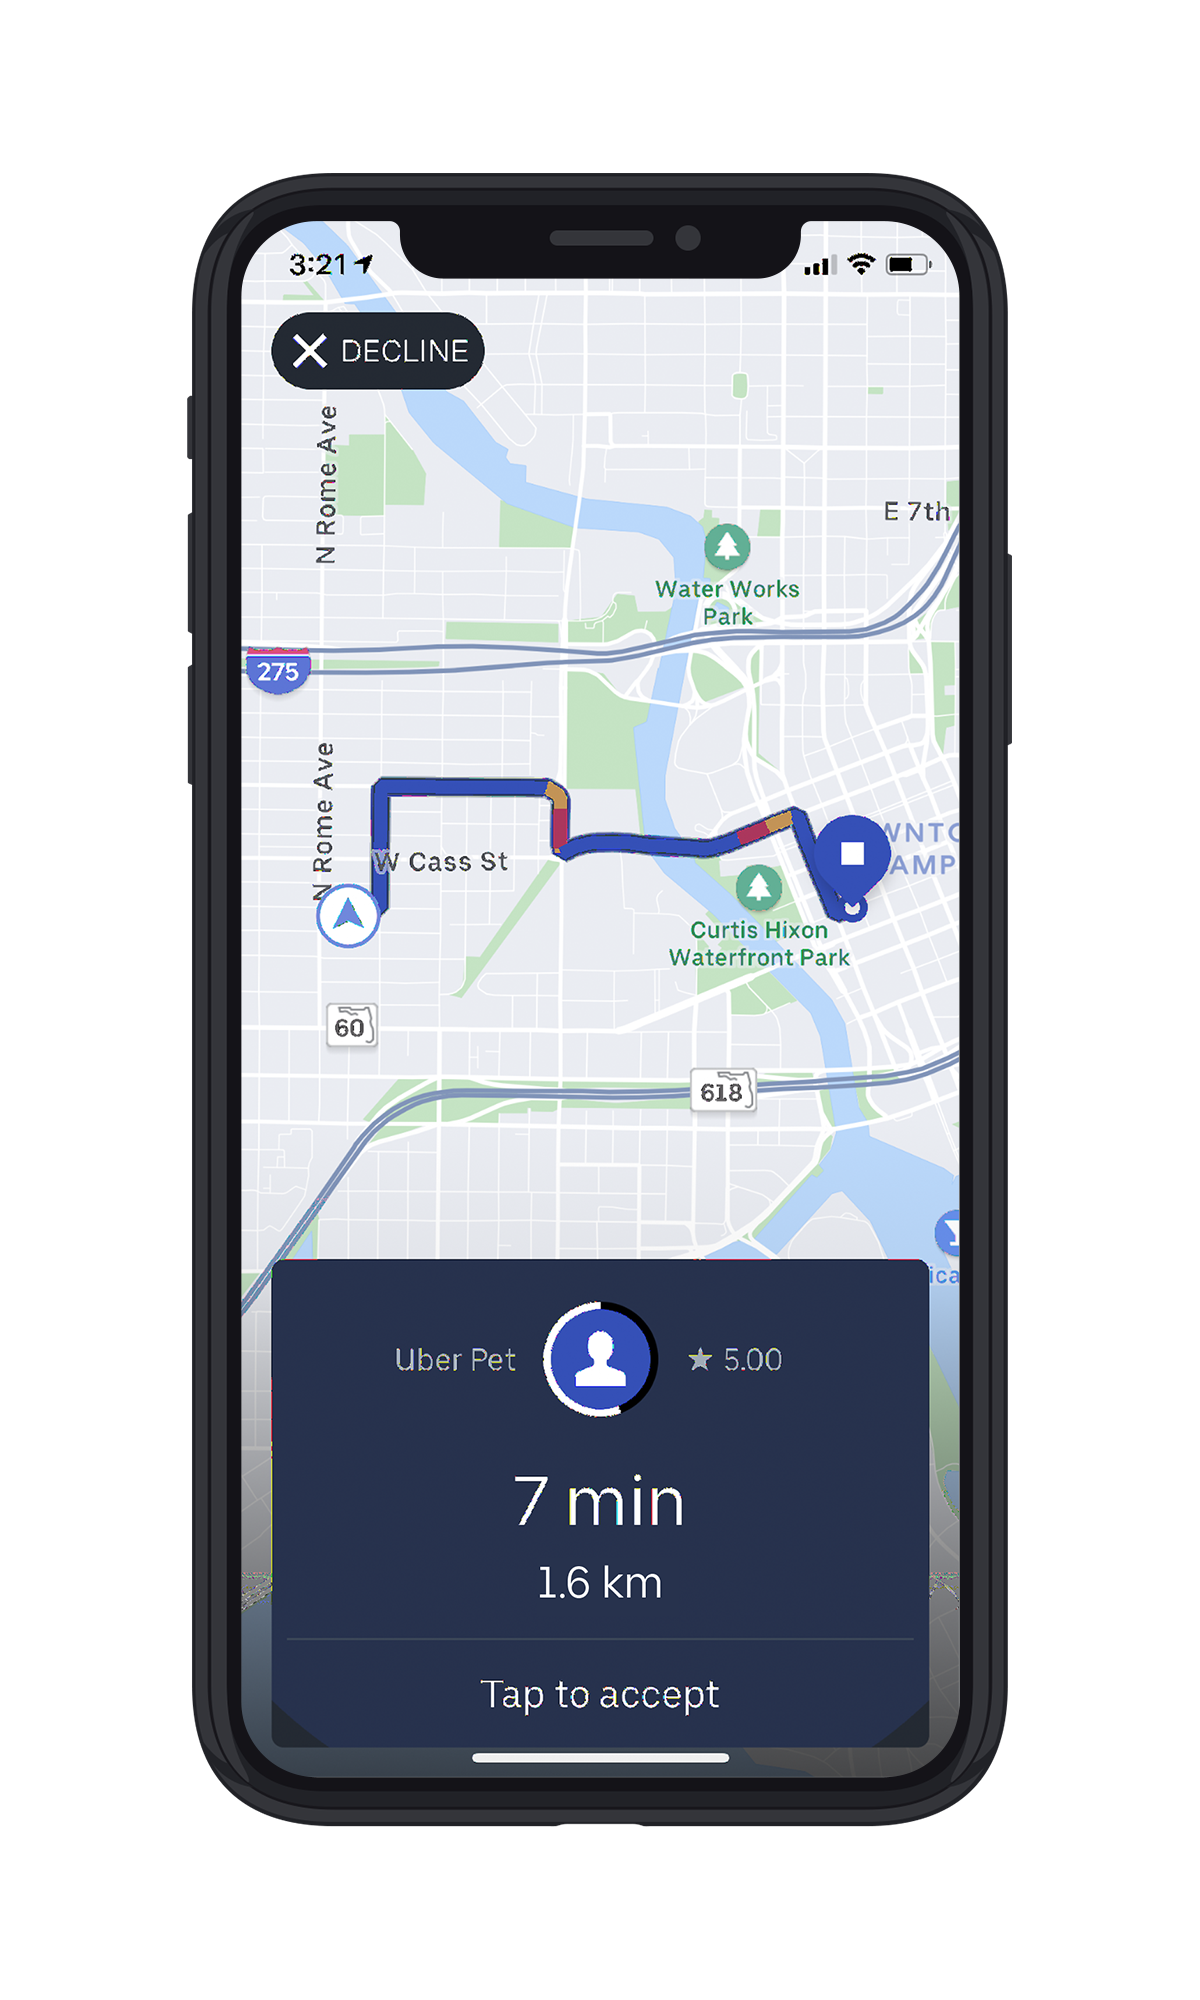
\includegraphics[width=0.4\textwidth]{Images/chapter1/uber.PNG}
    \caption{Uber}
    \label{fig:Application}
\end{figure}

\subsection{Samsung Health}
Samsung Health, à l'origine S Health, est une application gratuite développée par Samsung qui sert à suivre différents aspects de la vie quotidienne comme l'activité physique, l'alimentation et le sommeil.

Certaines fonctionnalités sont suivies par les entrées de l'utilisateur (nourriture / calories, poids, quantité d'eau, etc ...), et d'autres fonctionnalités sont suivies par des tests avec des accessoires de téléphone (Fitbit, Galaxy Active, Galaxy Fit, etc.) ou avec des capteurs de téléphone L'accéléromètre par exemple mesure l'accélération  dans de nombreux cas, par exemple: quand l'utilisateur fait du sport ou conduit sa voiture…

\textbf{Comment l'application mesure-t-elle les pas?}
Le smartphone détecte en permanence les mouvements du corps sur un accéléromètre à 3 axes. Les données sont enregistrées tout le temps qu'elles sont portées et allumées, ce qui permet au traqueur de suivre si l'individu marche en avant, court vite ou même immobile.

Les données collectées sont exécutées via un algorithme personnalisé. Cela permet au logiciel de détecter ce qu'impliquent réellement les différents mouvements enregistrés.

L'application permet à l'individu de savoir combien de pas ont été faits, à quelle vitesse, le rythme de l'individu, et même le nombre de calories susceptibles d'avoir été brulées. L'application permet à l'individu d'interagir avec les informations d'une manière conviviale.

\begin{figure}[h!]
    \center
    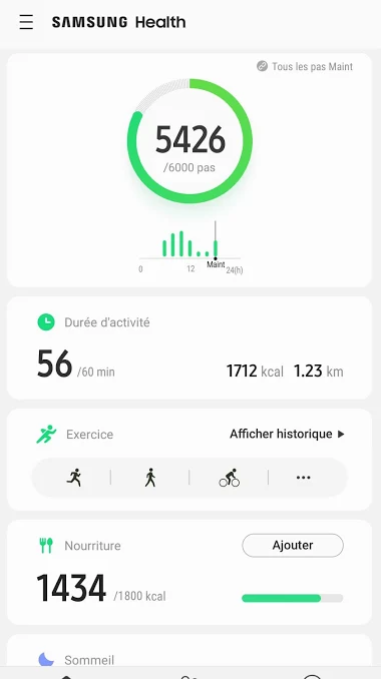
\includegraphics[width=0.33\textwidth]{Images/chapter1/samsungHealth.png}
    \caption{Samsung Health}
    \label{fig:Application}
\end{figure}
